\documentclass{beamer}

\usepackage[utf8]{inputenc}

\usepackage{alltt}
\usepackage{xcolor}
\usepackage[overlay,absolute]{textpos}
\usepackage[normalem]{ulem}

\usepackage{tikz}
\usetikzlibrary{arrows,petri,topaths}
\usepackage{tkz-berge}

%% Colors for source highlighting
\definecolor{scKW}  {HTML}{AA37F2}
\definecolor{scFct} {HTML}{1010FF}
\definecolor{scType}{HTML}{228B22}
\definecolor{scVar} {HTML}{A45936}
\definecolor{scComm}{HTML}{B32525}

%% Define _s_cala commands
\newcommand{\sK}[1]{{\color{scKW} #1}}
\newcommand{\sF}[1]{{\color{scFct} #1}}
\newcommand{\sV}[1]{{\color{scVar} #1}}
\newcommand{\sT}[1]{{\color{scType} #1}}
\newcommand{\sC}[1]{{\color{scComm} #1}}
\newcommand{\sH}[1]{{\color{white} #1}}
\newcommand{\sN}[1]{{\color{black} #1}}
\newcommand{\sS}{\vspace{0.8mm}}
\newcommand{\sEL}{\vspace{\baselineskip}}

%% Define other commands
\newcommand<>{\strike}[1]{\alt#2{\sout{#1}}{#1}}

\setbeamercovered{transparent}
\setbeamertemplate{navigation symbols}

\setbeamertemplate{footline}{\makebox[0.98\paperwidth][r]{\large
    \raisebox{1.2ex}{\insertframenumber}}}

\graphicspath{{figs/}}

\title{FlowArrays}
\subtitle{Barrier-Free ParArrays}

\author{Tobias Schlatter}
\date{January 17, 2012}
\institute{Advisors: Heather Miller, Aleksandar Prokopec, Philipp Haller and Martin Odersky}

\begin{document}

\begin{frame}
  \titlepage
\end{frame}

\section{Introduction}

\begin{frame}
  \frametitle{Outline}
  
  \begin{block}{What is a FlowArray}\end{block}
  \begin{block}{Task Scheduling}\end{block}
  \begin{block}{Benchmarks}\end{block}

\end{frame}

\section{What is a FlowArray}

\begin{frame}
  \frametitle{What is a FlowArray}
  \framesubtitle{Big Picture}

  \begin{columns}[t]
    \column{.5\textwidth}

    FlowArray: Barrier-Free, single-assignment ParArray

    \vspace{\baselineskip}

    \begin{block}{FlowArray Properties}
      \begin{itemize}
      \item<1> IndexedSeq semantics
      \item<2,3> Asynchronous
      \item<4> Deterministic
      \item<5> Lock-Free
      \end{itemize}
    \end{block}

    \column{.5\textwidth}

    \begin{overprint}
      \onslide<1>
      \begin{block}{IndexedSeq semantics}
        \begin{itemize}
        \item Immutable
        \item Ordered
        \item Fixed size
        \item Monadic operations\\
          \texttt{map}, \texttt{fold}, \texttt{flatMap}, etc.
        \end{itemize}
      \end{block}

      \onslide<2>
      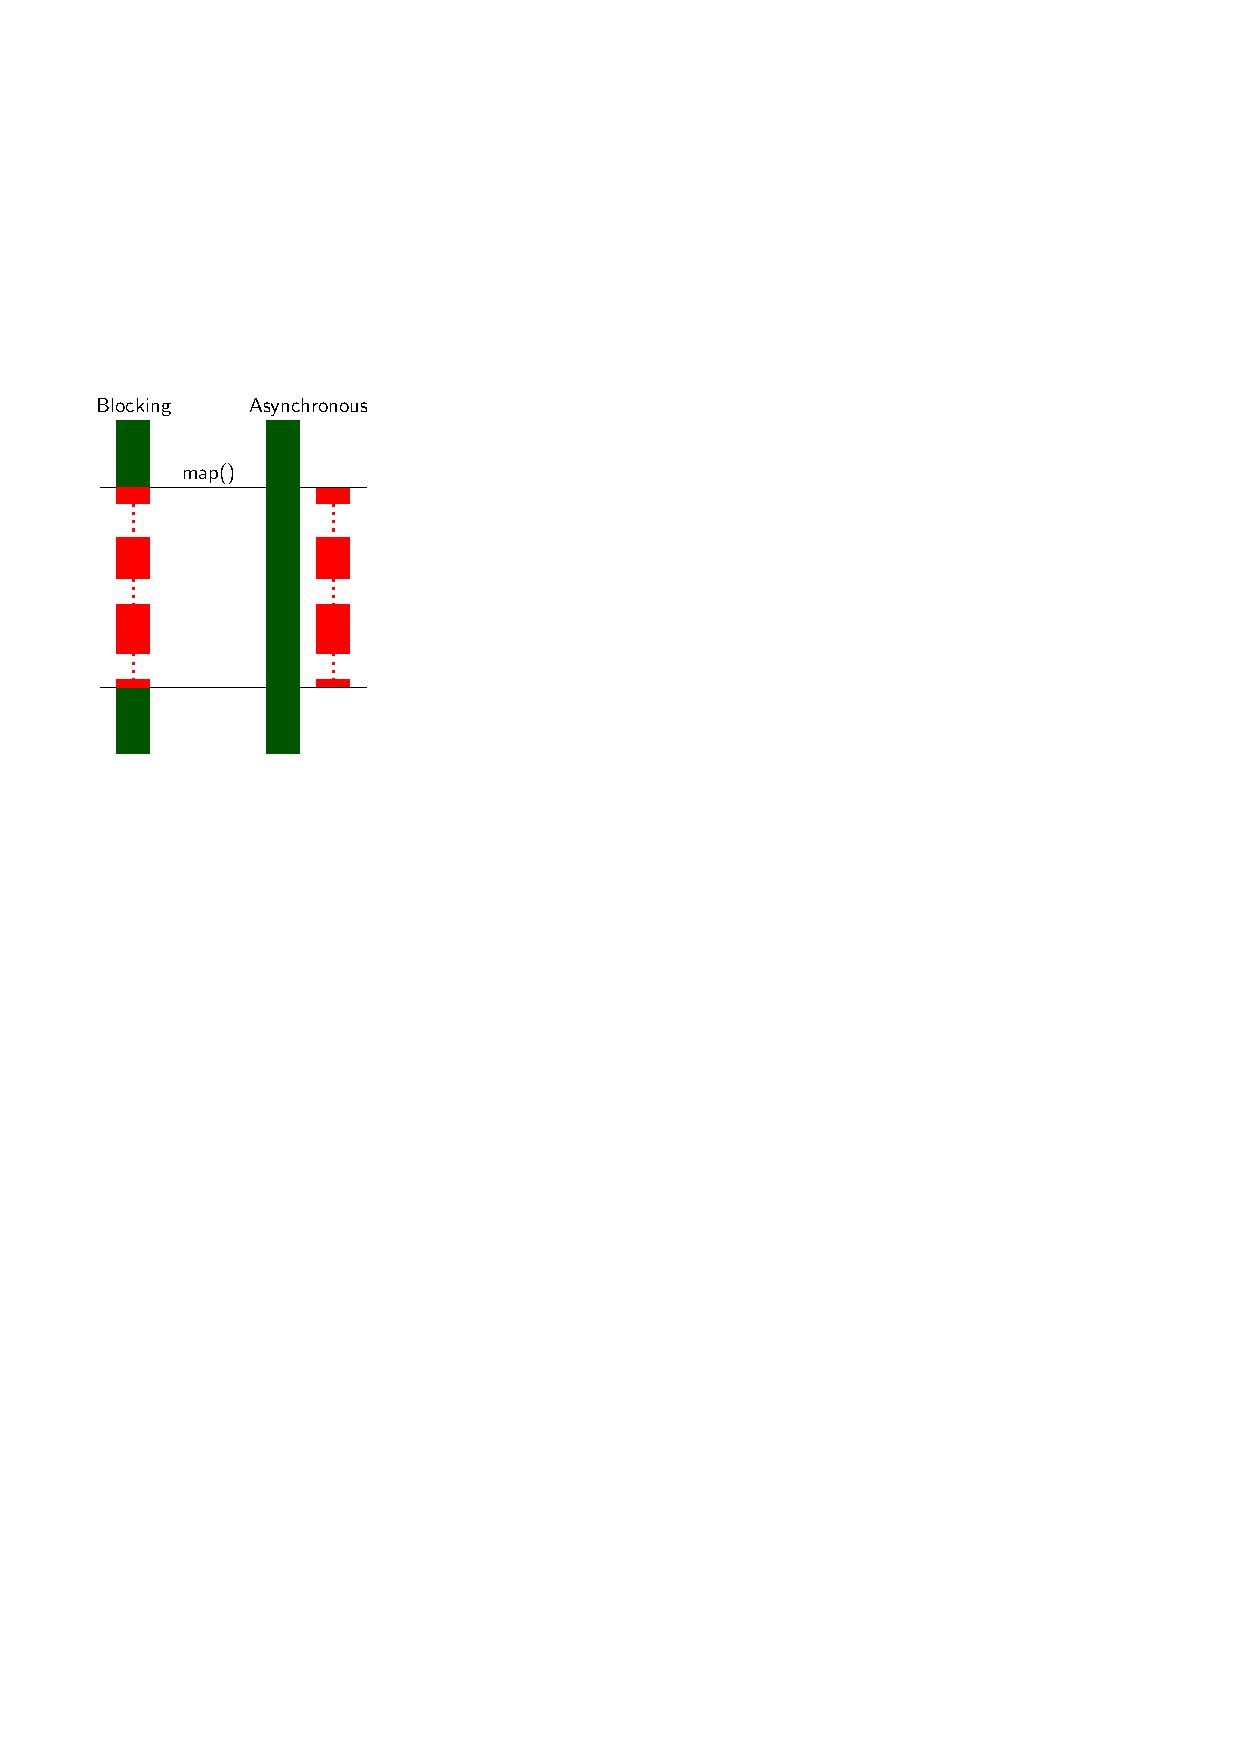
\includegraphics[page=1]{async}

      \onslide<3>
      \includegraphics[page=2]{async}

      \onslide<4>
      \begin{block}{Determinism}
        Every execution of a given program with given input eventually
        \begin{itemize}
        \item Always reaches same state
        \item[] \qquad or
        \item Always fails
        \end{itemize}
      \end{block}

      \onslide<5>
      \begin{block}{Locking}
        \begin{alltt}
          \sK{synchronized} \{\\
          \sH{xx}i = i + 1\\
          \}
        \end{alltt}
      \end{block}

      \begin{block}{Lock-Free}
        \begin{alltt}
          \sK{do} \{\\
          \sH{xx}ov = READ(i)\\
          \sH{xx}nv = ov + 1\\
          \} \sK{while} (!CAS(i, ov, nv))
        \end{alltt}
      \end{block}

    \end{overprint}
  \end{columns}
\end{frame}

\begin{frame}
  \frametitle{What is a FlowArray}
  \framesubtitle{Programming Model}

  \begin{alltt} \small
    \sC{// Generation}\\
    \sK{def} \sF{tabulate}[\sT A](\sV n: \sT{Int})(\sV f: \sT{Int => A}): \sT{FlowArray[A]}\\
    \sEL
    \sC{// Monadic Ops}\\
    \sK{def} \sF{map}[\sT B](\sV f: \sT{A => B}): \sT{FlowArray[B]}\\
    \sK{def} \sF{zip}[\sT B](\sV{that}: \sT{FlowArray[B]}): \sT{FlowArray[(A,B)]}\\
    \sK{def} \sF{fold}[\sT{A1 >: A}](\sV z: \sT{A1})(\sV{op}: \sT{(A1, A1) => A1}): \sT{Future[A1]}\\
    \sK{def} \sF{flatMapN}[\sT B](\sV n: \sT{Int})(\sV f: \sT{A => FlowArray[B]}): \sT{FlowArray[B]}\\
    \sK{def} \sF{flatten}[\sT B](\sV n: \sT{Int}): \sT{FlowArray[B]}\\
    \sEL
    \sC{// Structure}\\
    \sK{def} \sF{slice}(\sV{start}: \sT{Int}, \sV{end}: \sT{Int}): \sT{FlowArray[A]}\\
    \sK{def} \sF{transpose}(\sV{dim}: \sT{Int}): \sT{FlowArray[A]}\\
    \sEL
    \sC{// Retrieval}\\
    \sK{def} \sF{blocking}: \sT{Array[A]}
  \end{alltt}

\end{frame}

\begin{frame}
  \frametitle{What is a FlowArray}
  \framesubtitle{Flow Graph for Scalar Product}

  \begin{columns}
    \begin{column}{.45\textwidth}

      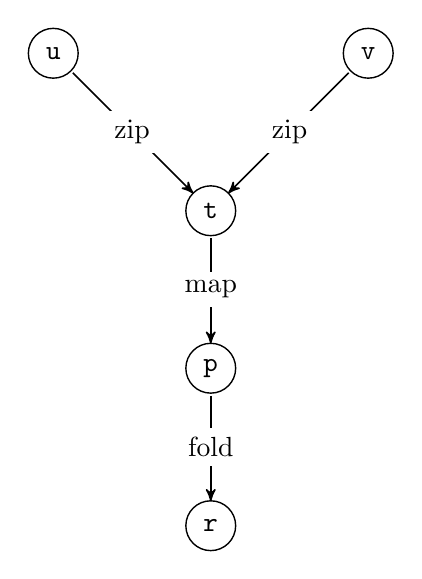
\begin{tikzpicture}[ node distance = 2cm ]
        \tikzset{EdgeStyle/.style={post}}       % directed edges

        \Vertex[x = 0, y = 7, L = \texttt{u}]{U}
        \Vertex[x = 4, y = 7, L = \texttt{v}]{V}

        \uncover<2->{
          \Vertex[x = 2, y = 5, L = \texttt{t}]{T}
          \Edge[label = zip](U)(T)
          \Edge[label = zip](V)(T)
        }

        \uncover<3->{
          \Vertex[x = 2, y = 3, L = \texttt{p}]{P}
          \Edge[label = map](T)(P)
        }

        \uncover<4->{
          \Vertex[x = 2, y = 1, L = \texttt{r}]{R}
          \Edge[label = fold](P)(R)
        }

        % \tikzset{EdgeStyle/.append style = {bend right}}

      \end{tikzpicture}  

    \end{column}

    \begin{column}{.55\textwidth}
      
      \begin{alltt} \small
        \sK{val} \sV u = FA.tabulate(n)(\_ * .9)\\
        \sK{val} \sV v = FA.tabulate(n)(\_ * .8)\\
        \sEL
        \uncover<2->{\sK{val} \sV t = u zip v}\\
        \uncover<3->{\sK{val} \sV p = t.map(\_ * \_)}\\
        \uncover<4->{\sK{val} \sV r = p.fold(0.0)(\_ + \_)}
      \end{alltt}

    \end{column}

  \end{columns}

\end{frame}


\section{Task Scheduling}

\begin{frame}
  \frametitle{Task Scheduling}
  \framesubtitle{ParArray --- \texttt{map}}

  \begin{alltt} \small
    \sK{val} \sV{pa1} = ParArray.tabulate(100)(x => x * x)\\
    \uncover<1,11->{\sK{val} \sV{pa2} = pa1.map(\_ * 2)}\\
    \uncover<1,14->{\sK{val} \sV{el}\sH{xx}= pa2(35)}
  \end{alltt}

  \vspace{\stretch{1}}

  \begin{overprint}
    \onslide<2>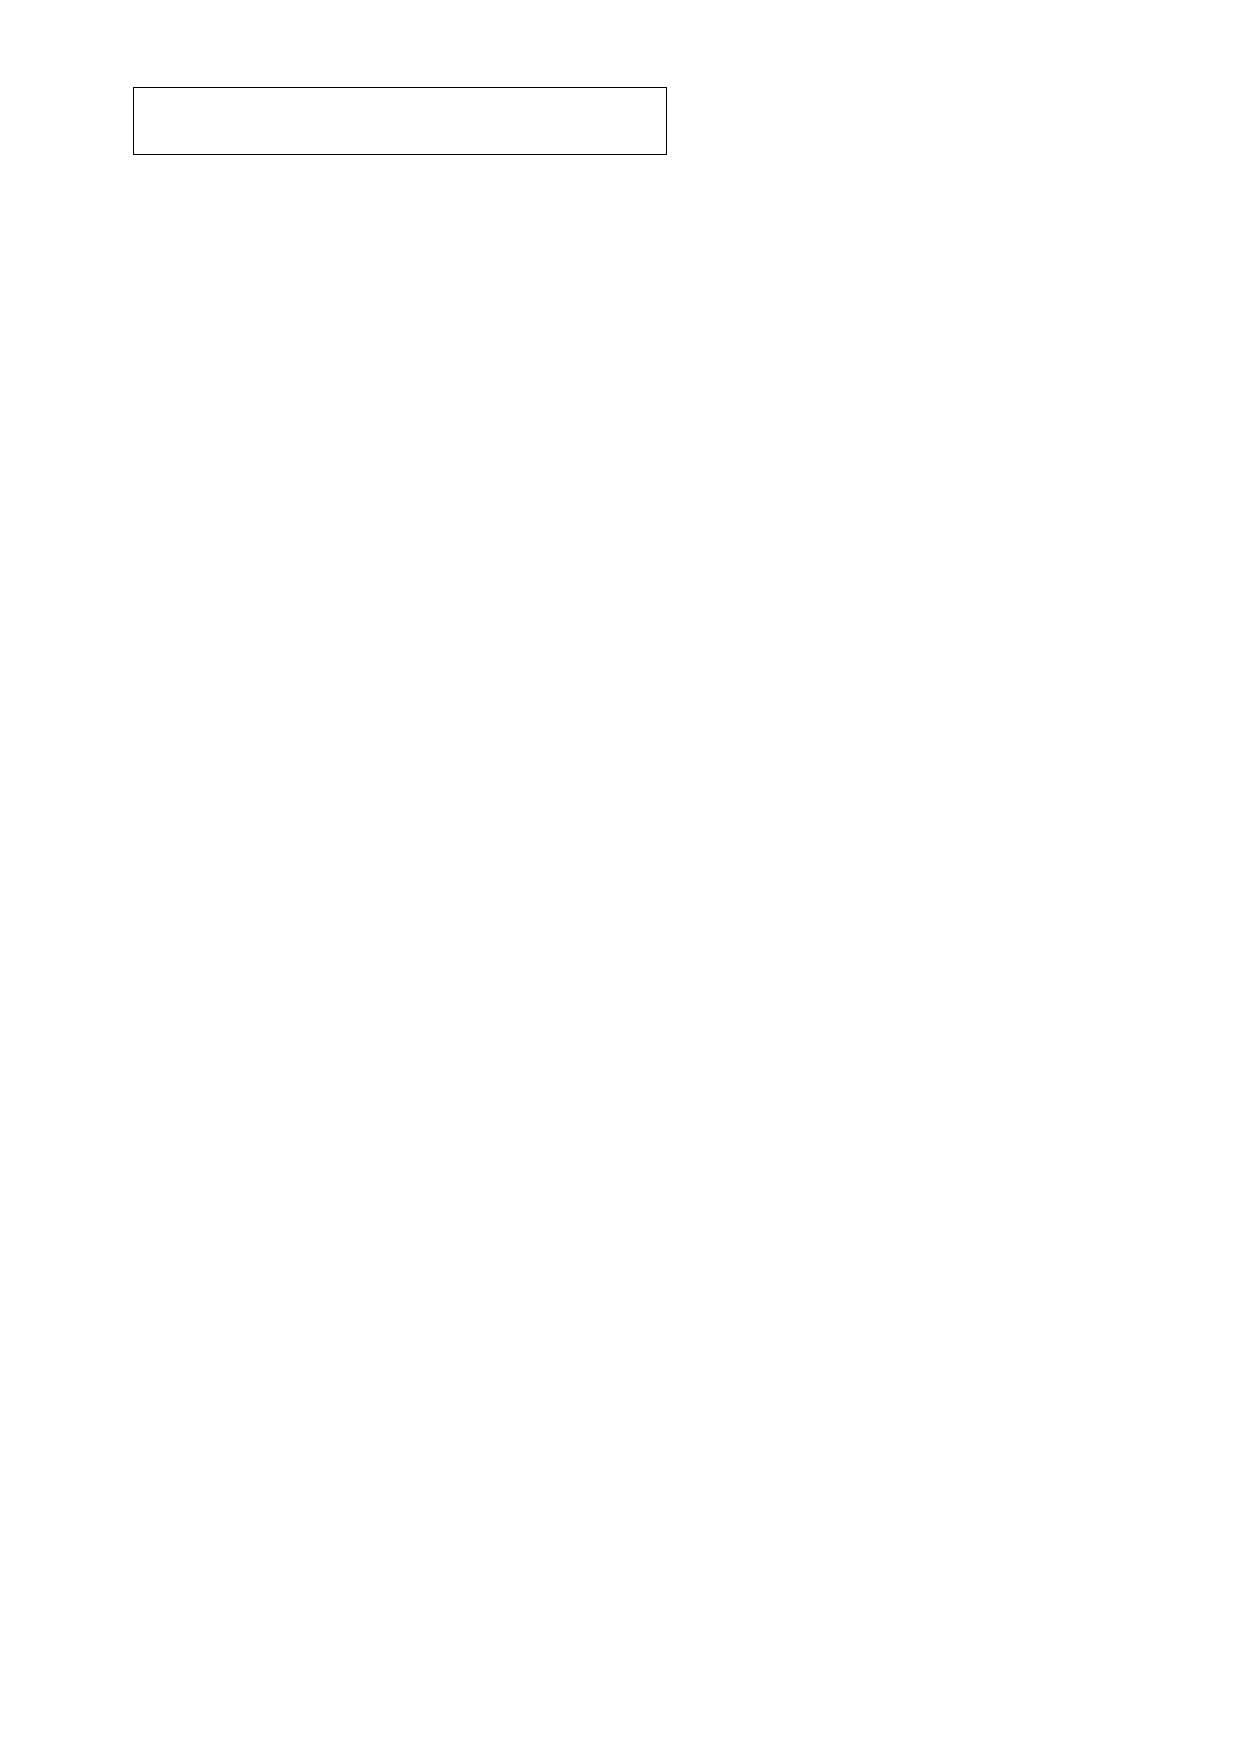
\includegraphics[page=1]{pa-map}
    \onslide<3>\includegraphics[page=2]{pa-map}
	\onslide<4>\includegraphics[page=3]{pa-map}
	\onslide<5>\includegraphics[page=4]{pa-map}
	\onslide<6>\includegraphics[page=5]{pa-map}
	\onslide<7>\includegraphics[page=6]{pa-map}
	\onslide<8>\includegraphics[page=7]{pa-map}
	\onslide<9>\includegraphics[page=8]{pa-map}
	\onslide<10>\includegraphics[page=9]{pa-map}
	\onslide<11>\includegraphics[page=10]{pa-map}
	\onslide<12>\includegraphics[page=11]{pa-map}
	\onslide<13->\includegraphics[page=12]{pa-map}
  \end{overprint}

\end{frame}



\begin{frame}
  \frametitle{Task Scheduling}
  \framesubtitle{FlowArray --- \texttt{map}}

  \begin{alltt} \small
    \sK{val} \sV{fa1} = FlowArray.tabulate(100)(x => x * x)\\
    \uncover<1,3->{\sK{val} \sV{fa2} = fa1.map(\_ * 2)}\\
    \uncover<1,5->{\sK{val} \sV{el}\phantom{xx}= fa2.blocking(35)}
  \end{alltt}

  \vspace{\stretch{1}}

  \begin{overprint}
    \onslide<2,3>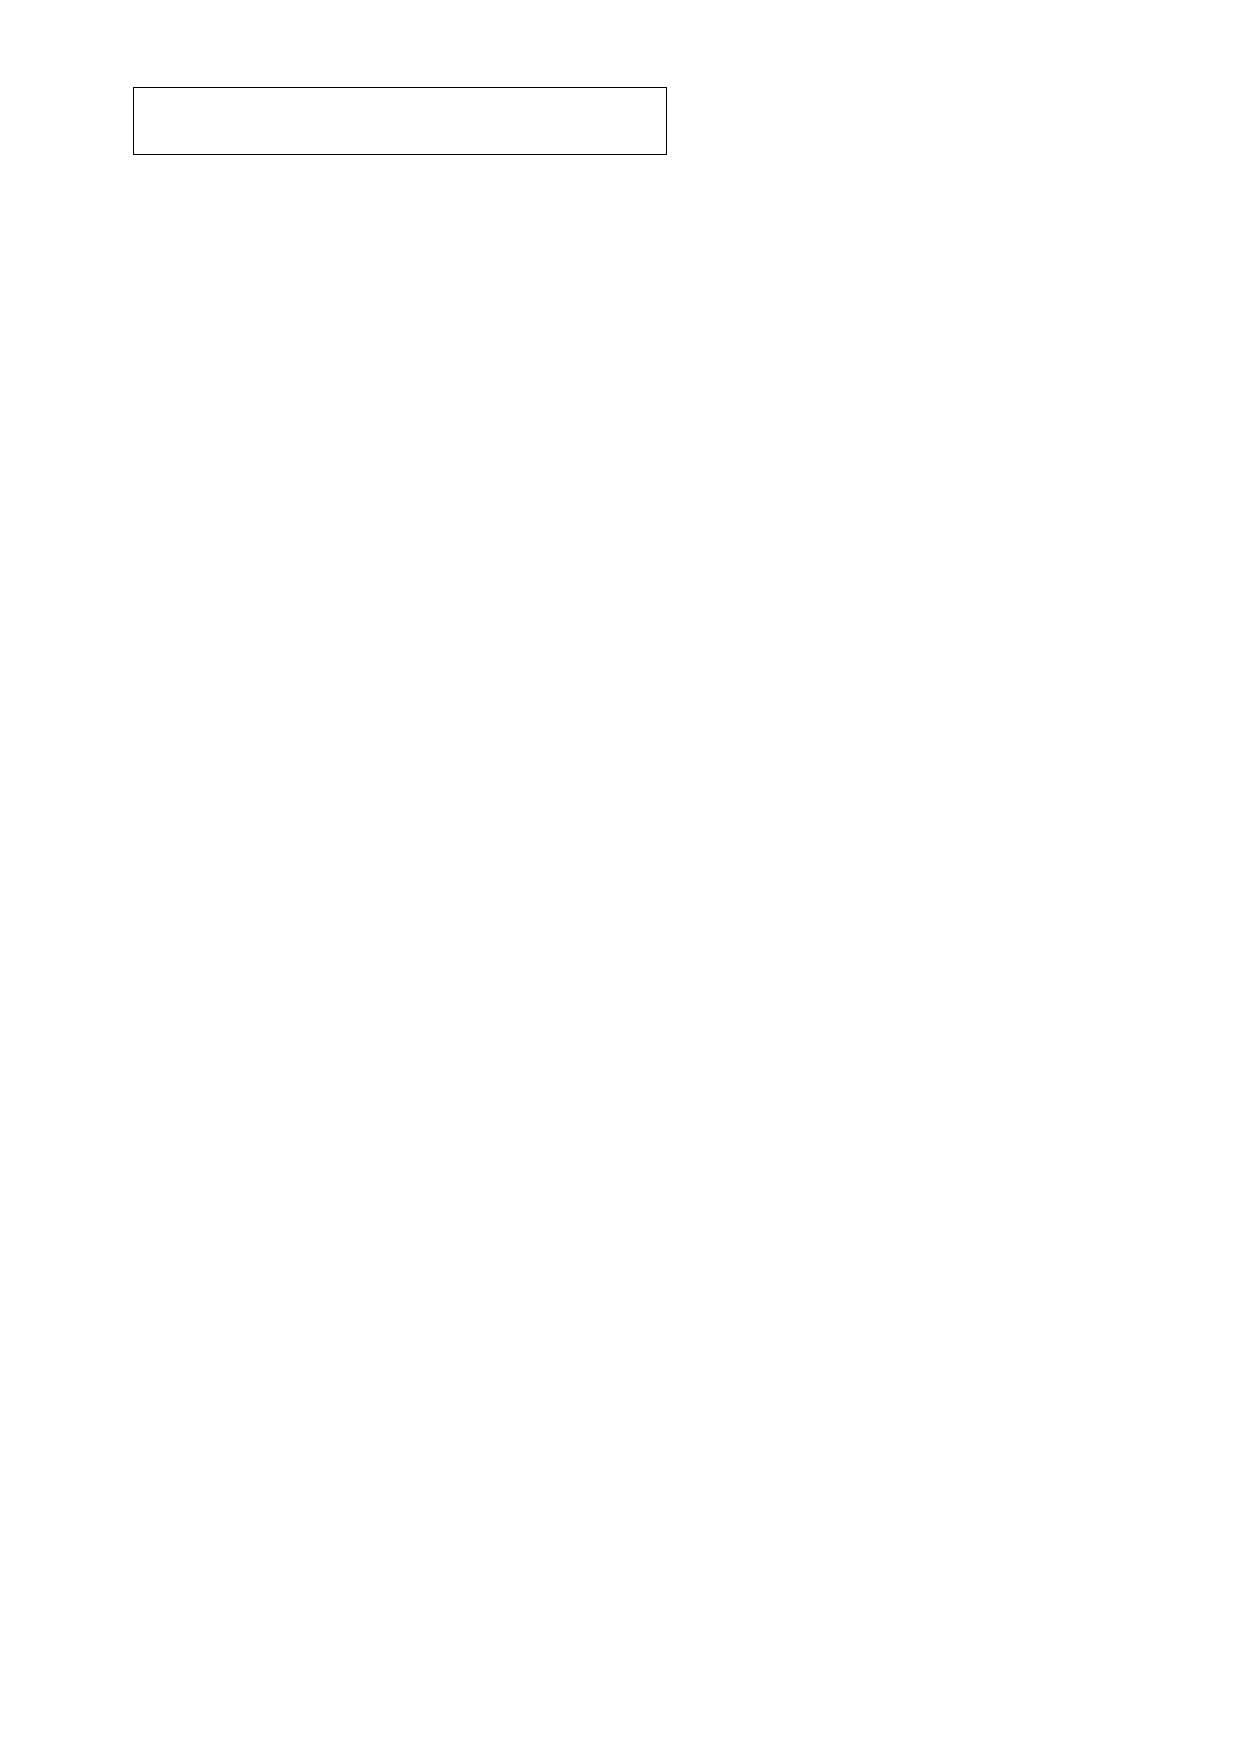
\includegraphics[page=1]{fa-map}
    \onslide<4>\includegraphics[page=2]{fa-map}
    \onslide<5>\includegraphics[page=3]{fa-map}
    \onslide<6>\includegraphics[page=4]{fa-map}
    \onslide<7>\includegraphics[page=5]{fa-map}
    \onslide<8>\includegraphics[page=6]{fa-map}
    \onslide<9>\includegraphics[page=7]{fa-map}
    \onslide<10>\includegraphics[page=8]{fa-map}
    \onslide<11>\includegraphics[page=9]{fa-map}
    \onslide<12>\includegraphics[page=10]{fa-map}
    \onslide<13>\includegraphics[page=11]{fa-map}
    \onslide<14>\includegraphics[page=12]{fa-map}
  \end{overprint}

\end{frame}

\begin{frame}
  \frametitle{Task Scheduling}
  \framesubtitle{FlowArray --- \texttt{fold}}

  \begin{alltt} \small
    \sK{val} \sV{res} = fa1.fold(0.0)(\_ + \_)
  \end{alltt}

  \vspace{\stretch{1}}

  \includegraphics<1>[page=1]{fa-fold}
  \includegraphics<2>[page=2]{fa-fold}
  \includegraphics<3>[page=3]{fa-fold}
  \includegraphics<4>[page=4]{fa-fold}
  \includegraphics<5>[page=5]{fa-fold}
  \includegraphics<6>[page=6]{fa-fold}
  \includegraphics<7>[page=7]{fa-fold}

\end{frame}

\section{Benchmarks}

\begin{frame}
  \frametitle{Benchmarks}
  \framesubtitle{Scalar Product -- Scaling / Garbage Collection}

  %% Hack to use whole frame
  \begin{columns}[t]
    \column{.33\paperwidth}
    \input{../../benchmarks/flowArrays/plots/pres-par-time.tex}
    \column{.32\paperwidth}
    \input{../../benchmarks/flowArrays/plots/pres-par-gctime.tex}
    \column{.35\paperwidth}
    \input{../../benchmarks/flowArrays/plots/pres-par-ntime.tex}
  \end{columns}

\end{frame}

\begin{frame}
  \frametitle{Benchmarks}
  \framesubtitle{Scalar Product -- Size / Garbage Collection}

  %% Hack to use whole frame
  \begin{columns}[t]
    \column{.33\paperwidth}
    \input{../../benchmarks/flowArrays/plots/pres-size-time.tex}
    \column{.32\paperwidth}
    \input{../../benchmarks/flowArrays/plots/pres-size-gctime.tex}
    \column{.35\paperwidth}
    \input{../../benchmarks/flowArrays/plots/pres-size-ntime.tex}
  \end{columns}

\end{frame}

\section{Conclusion}

\begin{frame}
  \frametitle{Conclusion}

  %% TODO

  \pause
  \begin{block}{¿Questions?}
  \end{block}

\end{frame}

\section{Appendix}

\begin{frame}
  \frametitle{Details about Benchmarks}

  \begin{columns}[t]
    \begin{column}{.5\textwidth}
      \begin{block}{Scaling}
        \begin{itemize}
        \item $10^7$ elements
        \item 20 measurements
        \end{itemize}
      \end{block}

      \begin{block}{Size}
        \begin{itemize}
        \item Parallelization level: 4
        \item 20 measurements
        \end{itemize}
      \end{block}

    \end{column}
    \begin{column}{.5\textwidth}
      \begin{block}{Java Command}
        \small\texttt{-Xmx2048m -Xms2048m -XX:+UseCondCardMark
          -verbose:gc -XX:+PrintGCDetails -server}.
      \end{block}
      \begin{block}{Arch, Java Version}
        Intel i7-2620M\\
        \small\texttt{
          Java 1.7.0\_04-b20\\
          HotSpot 64-Bit Server VM (build 23.0-b21, mixed mode)
        }
      \end{block}
    \end{column}
  \end{columns}
    
\end{frame}

\end{document}

%%% Local Variables: 
%%% mode: latex
%%% TeX-master: t
%%% End: 
